\documentclass[t, notes, xcolor=table]{beamer}

\usepackage{wrapfig}
\usepackage{float}
% For tabs in verbatim
\usepackage{fancyvrb}

% Adjust position of the image
\usepackage[export]{adjustbox}

% set fonts
\usefonttheme{professionalfonts} % using non standard fonts for beamer
\usepackage{txfonts,mathptmx}

% set indend spacing for first and second level indentation
\setlength{\leftmargini}{0.5cm}
\setlength{\leftmarginii}{0.5cm}
\setlength{\leftmarginiii}{0.5cm}

% Set circles for bullets 
\setbeamertemplate{itemize items}[circle]

% colors
\usepackage{xcolor}

% multiple columns
\usepackage{multicol}

% todo lists
\usepackage{pifont}
\usepackage{amssymb}

% increase space between text and frame name
\addtobeamertemplate{frametitle}{}{\vspace{0.5em}}

%Information to be included in the title page:
\title{Making Procedural Statements}
\author{Nikola Petrovic}
\institute{University of Belgrade, School of Electrical Engineering}
\date{2022}



\begin{document}

\frame{\titlepage}

%%%%%%%%%%%%%%%%%%%%%%%%%%%%%%%%%%%%%%%%%%%%%%%%%%%%%%%%%%%%
\begin{frame}
\frametitle{Module Objective}

In this module we will describe design behaviour procedurally.
\textbf{Topics:}
\begin{itemize}
\item Procedural blocks review
\item Making procedural statements
\item Making conditional statements
\item Making case statements
\item Making loop statements
\end{itemize}

\end{frame}
\note{
Out objective is to appropriately and effectively procedurally describe design behaviour. To do that, we need to know generally about procedural blocks and procedural statements, and more specifically about branching procedural statements. The Verilog behavioural modeling constructs are very similar to the C programming language. They differ in subtle ways that can sometimes be irksome.
}

%%%%%%%%%%%%%%%%%%%%%%%%%%%%%%%%%%%%%%%%%%%%%%%%%%%%%%%%%%%%
\begin{frame}
\frametitle{Describing Module Behaviour}

\begin{itemize}
\item The \textcolor{purple}{initial} construct starts execution at the start of the simulation, and when complete, terminates the process.
\item The \textcolor{purple}{always} construct starts execution at the start of the simulation, and when complete, executes again.

\begin{figure}
    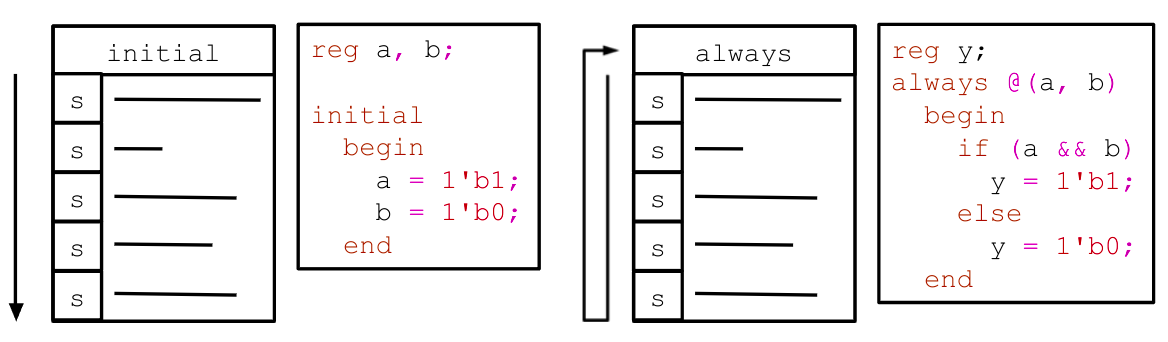
\includegraphics[width=0.95\textwidth]{img/06_mod_beh.png}
\end{figure}
\end{itemize}
\end{frame}
\note{
\scriptsize{
Event simulation relies upon processes. A process is an object that reacts to input events and generates output events. The continuous assignment that we have already seen is a process - the simulator reacts to its input transitions to calculate new output value and transitions the net to that new value.
\newline

Verilog has other kinds of processes - two most obvious to the user are the \textbf{initial} construct and the \textbf{always} construct, frequently referred to as the initial and the always block. The \textit{initial} and \textit{always} keywords are not statements themselves - they apply to their following statement and make it execute as a process. Their following statement is usually a statement block, e.g., statements between the \textit{begin} and \textit{end} keywords, but does not have to be.
\begin{itemize}
\item The simulator executes each \textit{initial} process at the start of the simulation, and upon completing its execution, terminates the process.
\item The simulator executes each \textit{always} process at the start of the simulation, and upon completing its execution, executes it again.
\end{itemize}

}
}

%%%%%%%%%%%%%%%%%%%%%%%%%%%%%%%%%%%%%%%%%%%%%%%%%%%%%%%%%%%%
\begin{frame}
\frametitle{Synchronizing Module Behaviours}
\scriptsize{
\begin{multicols}{2}
\begin{itemize}
\item Procedures "block" upon encountering an event control
\item Procedures "unblock" upon occurrence of any of the listed events.
\item An event control can reference:
\begin{itemize}
\scriptsize{
	\item A single event identifier
	\item An event expression
	\item The "$*$" wildcard operator
}
\end{itemize}

\end{itemize}
\vfill
\columnbreak
\begin{figure}
    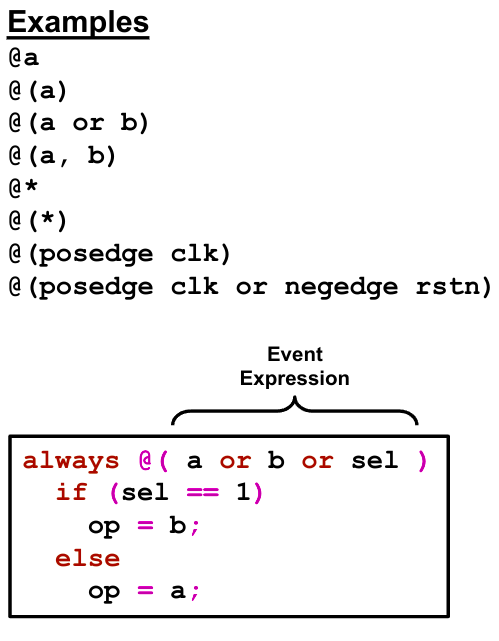
\includegraphics[width=0.45\textwidth]{img/06_sync.png}
\end{figure}
\end{multicols}
}
\end{frame}
\note{
\scriptsize{
If an \textbf{always} construct has no constructs to block it execution, then when the simulator started executing it at the start of simulation, execution would continue in a tight loop forever and the simulator would appear to hang.
\newline

Verilog provides procedural timing controls for "stepping" execution of procedural blocks. The most common of these is the event control. An event control starts with the \textbf{at (@)} character and then follows with either a wildcard character, a single event identifier, or a parenthesized event expression. The event expression can be a list of event expressions separated by the \textbf{or} keyword or by the comma (,) character. Both are shown in the example. The \textbf{or} keyword in an event expression is a separator between event expressions and is not an operator in the usual sense. We can further qualify an expression with the \textbf{posedge} or \textbf{negedge} keywords.
\newline

A timing control is not itself a statement, but precedes a statement, and in the case of an event control, blocks execution of that statement and subsequent sequential statements until on of those events occur.

}
}


%%%%%%%%%%%%%%%%%%%%%%%%%%%%%%%%%%%%%%%%%%%%%%%%%%%%%%%%%%%%
\begin{frame}
\frametitle{Interactions Between Behaviours}
\begin{figure}
    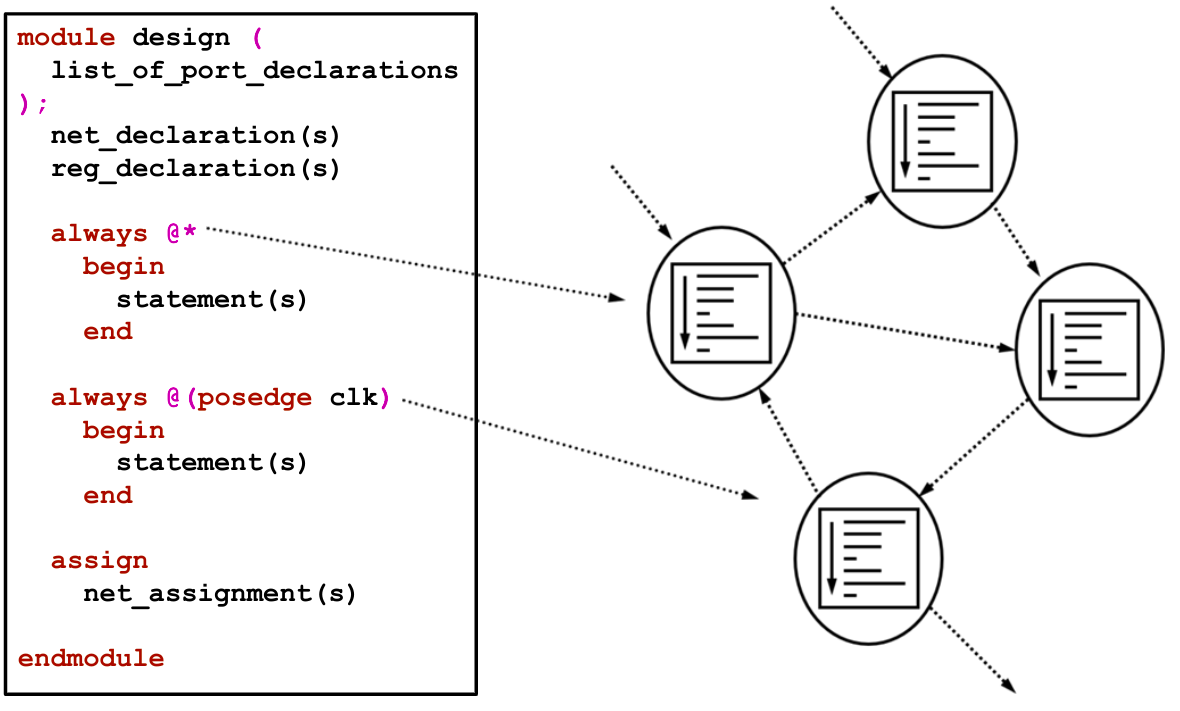
\includegraphics[width=0.95\textwidth]{img/06_interaction.png}
\end{figure}
\end{frame}
\note{
\scriptsize{
A non-trivial design usually contains several modules, and a module at the RT level typically contains procedural blocks:
\begin{itemize}
\item Each sequential procedural block executes its statement sequentially like a conventional programming language.
\item Multiple blocks execute concurrently, like hardware.
\item Multiple blocks communicate with each other using events, nets and variables.
\end{itemize}

The capability to have many procedural blocks communicating concurrently with each other is the basic model which Verilog uses to describe hardware.
}
}

%%%%%%%%%%%%%%%%%%%%%%%%%%%%%%%%%%%%%%%%%%%%%%%%%%%%%%%%%%%%
\begin{frame}
\frametitle{Making Procedural Assignments}
\scriptsize{
\begin{multicols}{2}
\begin{itemize}
\item Procedural assignments are assignments made inside procedures
\item We make procedural assignments only to variables!
\end{itemize}
\vfill
\columnbreak
\begin{figure}
    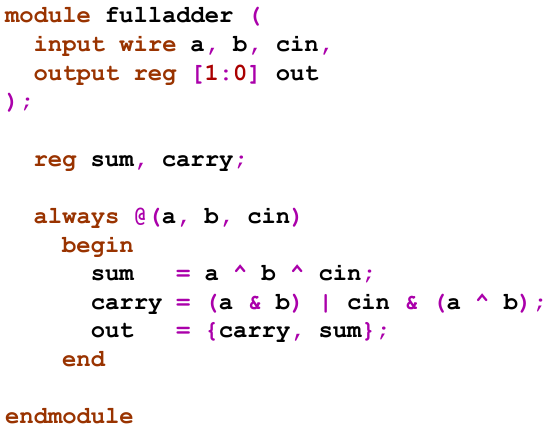
\includegraphics[width=0.45\textwidth]{img/06_make_assign.png}
\end{figure}
\end{multicols}
}
\end{frame}
\note{
\scriptsize{
The \textbf{initial} construct and the \textbf{always} construct are frequently referred to as \textbf{procedural blocks}, though as we have seen, whey can apply to an atomic statement. Statements within a \textit{procedural block} are procedural statements, and most of our procedural statements will be assignments.
\begin{itemize}
\item Recall that a continuous assignment is to a net and is its own process, so only exists \textbf{outside} any procedural blocks.
\item A procedural assignment is to a variable and is not its own process, so only exists \textbf{inside} a procedural block.
\item The right operand of either assignment can contain constants, variables and nets, as on the right side only their values are used.
\end{itemize}

}
}

%%%%%%%%%%%%%%%%%%%%%%%%%%%%%%%%%%%%%%%%%%%%%%%%%%%%%%%%%%%%
\begin{frame}
\frametitle{Making Conditional Statements}
\scriptsize{
\begin{multicols}{2}
\begin{itemize}
\item \textbf{if} is a conditional statement
\item \textbf{if} tests the condition in sequence
\item Conditions can overlap
\item Executes statement associated with first known true condition
\item Statement can be null ";"
\end{itemize}
\vfill
\columnbreak
\begin{figure}
    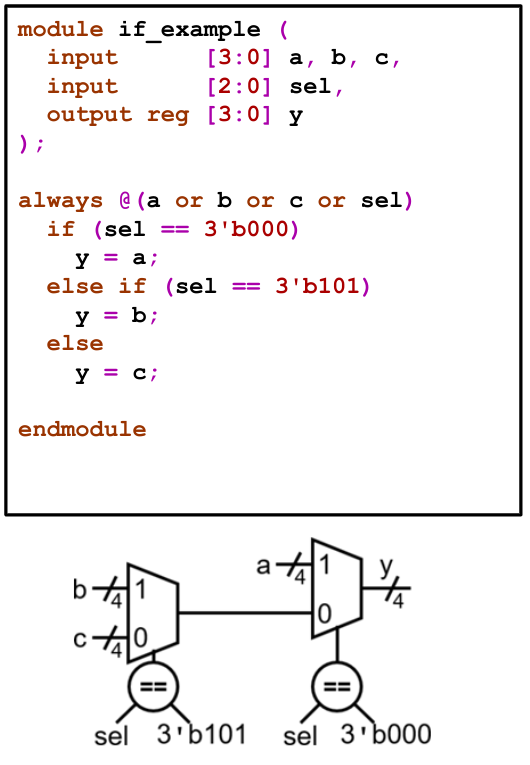
\includegraphics[width=0.45\textwidth]{img/06_cond.png}
\end{figure}
\end{multicols}
}
\end{frame}
\note{
\tiny{
\textbf{if} statement syntax:

if (expression)

\ \ statement
  
[\{else if (expression)

\ \ statement\}]
  
[else statement]
\newline

The conditional statement is a two-way branch. I the conditional expression evaluates to a known non-zero value then the first branch executes and otherwise the second branch executes if it exists. The conditional expression can be multiple bits.
\newline

As with other programming languages, in nested conditional statements, every \textbf{else} keyword is associated with the nearest previous \textbf{if} keyword that does not already have an \textit{else} associated with it. If this association displeases us, then we can force association by using \textbf{begin-end} sequential blocks, or we can just toss in the else keyword where needed with a null following statement.
\newline

In this example, execution of the procedural block blocks at the event control until a transition occurs on a least one of the module inputs. When a transition occurs, the conditional statement executes. It evaluates the \textit{sel} signal. if the value is exactly 3'b000, then it executes the first branch, which is an assignment of a to y. If the value is anything else, it executes the second branch, which is another conditional statement. This conditional statement again evaluates the sel signal. if the value is less than or equal to 3'b101, then it executes first branch, otherwise it executes the second branch. Note that such a chain of conditional statements implies priority. If the \textit{sel} signal is exactly 3'b000, then the second test for less than 3'b101 is not made, even though the value would match that second test if it were made.

}
}

%%%%%%%%%%%%%%%%%%%%%%%%%%%%%%%%%%%%%%%%%%%%%%%%%%%%%%%%%%%%
\begin{frame}
\frametitle{Conditional Statement Syntax}
\scriptsize{
\begin{multicols}{2}
\begin{figure}
    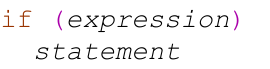
\includegraphics[width=0.25\textwidth, left]{img/06_cond_syn0.png}
\end{figure}
\vfill
\columnbreak
\textcolor{purple}{if} branch executes if condition is known true.
\end{multicols}
\begin{multicols}{2}
\begin{figure}
    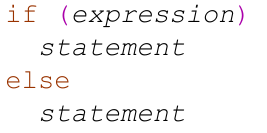
\includegraphics[width=0.25\textwidth, left]{img/06_cond_syn1.png}
\end{figure}
\vfill
\columnbreak
\textcolor{purple}{if} branch executes if condition is known true. \textcolor{purple}{else} branch executes if condition is false or unknown.
\end{multicols}
\begin{multicols}{2}
\begin{figure}
    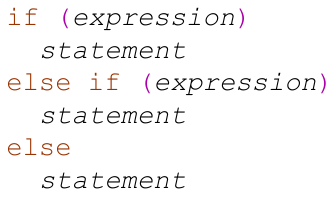
\includegraphics[width=0.32\textwidth, left]{img/06_cond_syn2.png}
\end{figure}
\vfill
\columnbreak
\textcolor{purple}{if} branch executes if condition  is known true. \textcolor{purple}{else if} branch executes for alternative condition known true. \textcolor{purple}{else} branch executes if no condition known true.
\end{multicols}
}
\end{frame}
\note{
The 1st illustration omits the second branch.
\newline

The 2nd illustration includes a new branch.
\newline

The 3rd illustration is not a new syntax. Unlike some programming languages, Verilog does not have the \textbf{elsif} keyword, so this is simply chaining two conditional statements.
}

%%%%%%%%%%%%%%%%%%%%%%%%%%%%%%%%%%%%%%%%%%%%%%%%%%%%%%%%%%%%
\begin{frame}
\frametitle{Making Case Statements: case}
\scriptsize{
\begin{multicols}{2}
\begin{itemize}
\item The \textcolor{purple}{case} statement is a multi-way prioritized branching statements.
\item \textcolor{purple}{case} item match expressions can overlap.
\item Compares item match expressions to case expression in the order that they appear.
\begin{itemize}
\scriptsize{
	\item uses case equality comparison
	\begin{itemize}
	\scriptsize{
		\item Bitwise 0,1,Z,X comparison	
	}
	\end{itemize}
	\item Executes statement associated with first match
	\item Executes optional default item if no other item matched
	\begin{itemize}
	\scriptsize{
		\item In this example, inputs containing Z or X	
	}
	\end{itemize}
}
\end{itemize}
\end{itemize}
\vfill
\columnbreak
\begin{figure}
    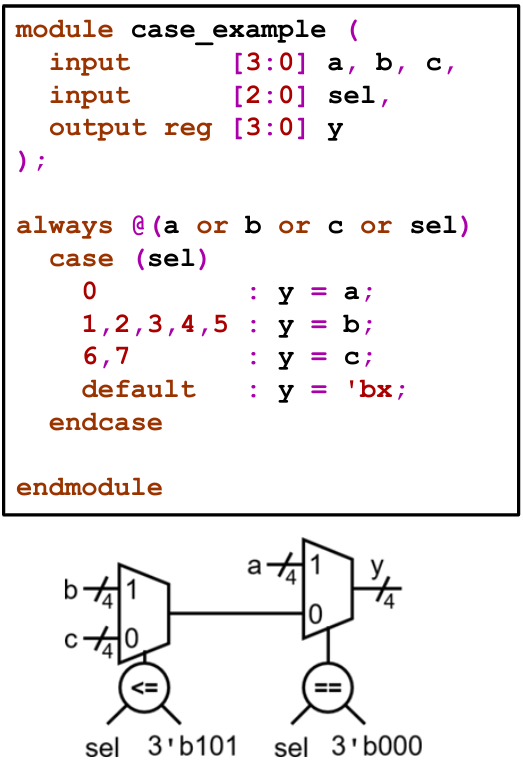
\includegraphics[width=0.45\textwidth]{img/06_case.png}
\end{figure}
\end{multicols}
}
\end{frame}
\note{
\tiny{
case (expression)

expression \{, expression\} : statement

\{expression \{, expression \} : statement \}

[default [:] statement]

endcase
\newline

The \textbf{case} statement is a multi-way prioritized branching statement. The case statement evaluates an expression and then evaluates a sequence of match expressions and executes the statement associated with only the first matching expression. 
The case statement considers high-impedance (z) and unknown (x) values and matches expressions that have a high-impedance or unknown bit in the same position in both expressions. We can comma separate multiple match expression associated with the same following statement. The following statement is often a statement block but does not have to be. We can optionally provide a \textbf{default} match item to be matched when no other match expression matches. it is common to place the default match item at the case statement end, but we can place it anywhere. We can have at most one default match item in each case statement.
\newline

In this example, execution of the procedural block is blocked at the event control until a transition occurs on at least on of the module inputs. When a transition occurs, the \textit{case} statement executes. It evaluates the "sel" signal. if the value is 0 then it executes the first branch. If the value is between 1 and 5 then it executes the second branch. If the value is between 6 and 7 then it executes the third branch. If the value is anything else, it executes the default branch, which sets the output unknown. As an unknown value does not infer any particular hardware, the hardware has no implementation of this default branch.

}
}


%%%%%%%%%%%%%%%%%%%%%%%%%%%%%%%%%%%%%%%%%%%%%%%%%%%%%%%%%%%%
\begin{frame}
\frametitle{Making Case Statements: casex}
\tiny{
\begin{multicols}{2}
Threats Z,X and ? characters as "don't care" bit positions in either:
\begin{itemize}
\item case expression (sel)
\item case item expression 3'b0XX
\end{itemize}
Lets you group match values for more concise description:
\begin{itemize}
\item Encoders, decoders, etc.
\item Not very useful in testbenches
\item Not a preferred method usually
\end{itemize}

\textcolor{purple}{casex} treats X in case expression as meaningful in uninitialized logic:
\begin{itemize}
\item Hides initialization problems
\item Not recommended!
\end{itemize}
\textcolor{purple}{casex} can't match unknown or high impedance values coming out of the DUT, so it's less useful in testbenches
\vfill
\columnbreak
\begin{figure}
    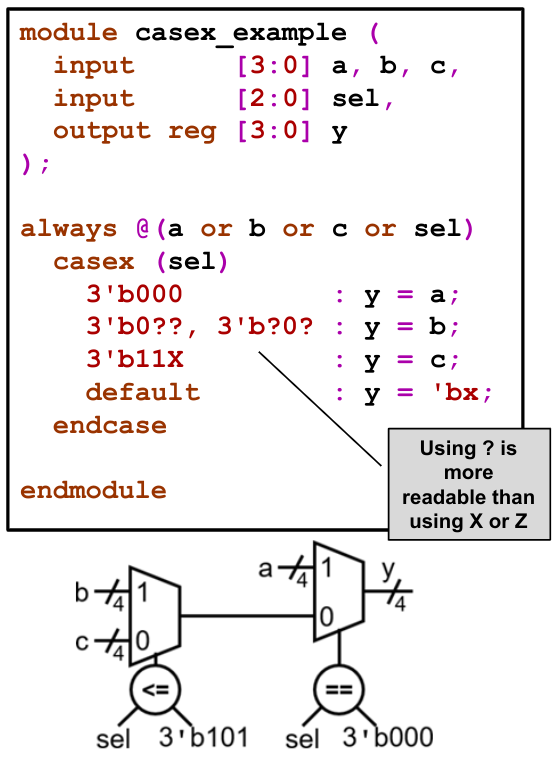
\includegraphics[width=0.45\textwidth]{img/06_casex.png}
\end{figure}
\end{multicols}
}
\end{frame}
\note{
\tiny{
The \textbf{casex} statement is a variation of the \textit{case} statement that lets you specify the bit positions it should not compare.
\newline

The \textit{casex} statement treats the x,z, and question mark (?) characters as \textit{don't care} bit values. Recall that in a literal constant the ? character is equivalent to the z character and that only the based literal constants can use the x,z, and ? characters.
\newline

The \textit{casex} statement does not compare bit positions of either the case expression or the case match items that have any of these "don't care" values.
\newline

By convention, we might want to use the ? character to indicate \textit{don't care} bit positions in literal constants to avoid confusion with the high-impedance and unknown values. However, the \textit{casex} statement still considers bit positions containing high-impedance (z) or unknown (x) values in expressions of nets and variables to be position it should not match, so a \textit{casex} statement in a testbench cannot test high-impedance or unknown values coming from the DUT.
\newline

This example is functionally identical to the previous example, but uses "don't care" bit positions to represent a range of matching values.

}
}

%%%%%%%%%%%%%%%%%%%%%%%%%%%%%%%%%%%%%%%%%%%%%%%%%%%%%%%%%%%%
\begin{frame}
\frametitle{Making Case Statements: casez}
\tiny{
\begin{multicols}{2}
Treat Z and ? characters as "don't care" bit positions in: 
\begin{itemize}
\item case expression (sel)
\item case item expression 3'b0ZZ
\end{itemize}
Performs definitive match for X
\begin{itemize}
\item useful in testbenches!
\end{itemize}
\textcolor{purple}{casez} is preferable to \textcolor{purple}{casex}
\begin{itemize}
\item X in case expression is not wildcard
\item Safer for uninitialized RTL code
\end{itemize} 
\vfill
\columnbreak
\begin{figure}
    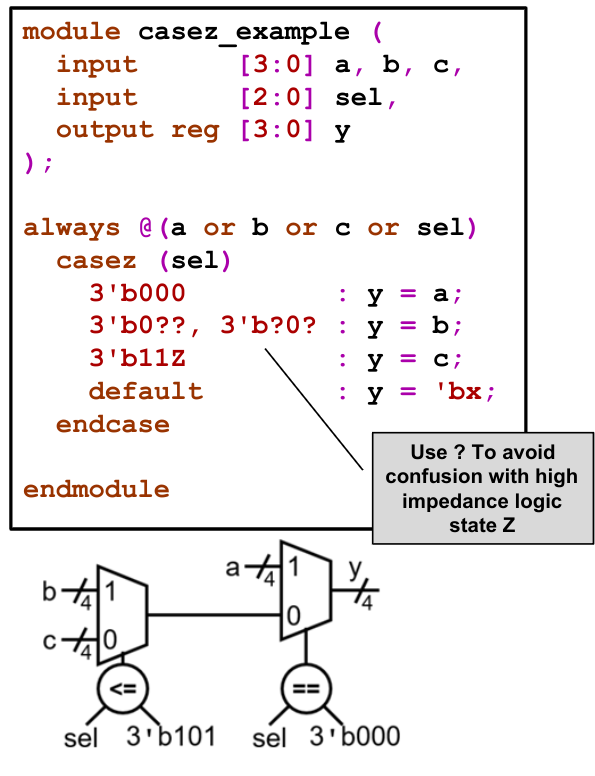
\includegraphics[width=0.45\textwidth]{img/06_casez.png}
\end{figure}
\end{multicols}
}
\end{frame}
\note{
\scriptsize{
The \textbf{casez} statement is a variation of the \textbf{casex} statement and treats only the z and question mark ? as "don't care" bit values and performs a definitive match for unknown (x) values. In a testbench, to test the existence of unknown values from the DUT, we should use the \textit{casez} statement instead of the \textit{casex} statement.
\newline

This example is functionally identical to the previous example, but uses the z character instead of the x character to represent the don't care bit positions.

}
}

%%%%%%%%%%%%%%%%%%%%%%%%%%%%%%%%%%%%%%%%%%%%%%%%%%%%%%%%%%%%
\begin{frame}
\frametitle{Alternative Case Statement Form}

\end{frame}

%%%%%%%%%%%%%%%%%%%%%%%%%%%%%%%%%%%%%%%%%%%%%%%%%%%%%%%%%%%%
\begin{frame}
\frametitle{Module}

\end{frame}

%%%%%%%%%%%%%%%%%%%%%%%%%%%%%%%%%%%%%%%%%%%%%%%%%%%%%%%%%%%%
\begin{frame}
\frametitle{Module}

\end{frame}

%%%%%%%%%%%%%%%%%%%%%%%%%%%%%%%%%%%%%%%%%%%%%%%%%%%%%%%%%%%%
\begin{frame}
\frametitle{Module}

\end{frame}

%%%%%%%%%%%%%%%%%%%%%%%%%%%%%%%%%%%%%%%%%%%%%%%%%%%%%%%%%%%%
\begin{frame}
\frametitle{Module}

\end{frame}

%%%%%%%%%%%%%%%%%%%%%%%%%%%%%%%%%%%%%%%%%%%%%%%%%%%%%%%%%%%%
\begin{frame}
\frametitle{Module}

\end{frame}

\end{document}
